\documentclass[12pt]{article}

\usepackage[margin=1in]{geometry}
\usepackage{setspace}
\usepackage{booktabs}
\usepackage{graphicx}
\usepackage{float}
\usepackage{hyperref}
\usepackage{enumitem}
\usepackage{amsmath}
\usepackage{listings}
\usepackage{xcolor}

\onehalfspacing

\title{
Final Project Problem\\
\large Masters of Applied Statistics and Data Science, Spring 2026
}
\author{Juan Cortes}
\date{\today}

\begin{document}

\maketitle

\section{Introduction}

We would like you to cover the following:

\begin{enumerate}
    \item What dataset did you use and what are the features in the dataset?
    \item What method(s) did you try to use and why did you select your final choice of method? Please explain the underlying principles of the technique that you used.
    \item Were there any considerations or choices you made with regards to missing data and or other data processing/cleaning?
     \item Were there any challenges you faced with your implementation?
     \item What are the outcomes of training your model? Was there a good fit? Did it work well with the training data? What was your accuracy score? Does it give good predictions?
\end{enumerate}

\section{Feature Overview}

The \href{https://www.kaggle.com/datasets/evilspirit05/affair-dataset/data}
{Marriage \& Affairs Dataset} dataset originally derived from a well-known behavioral study, aiming to uncover the underlying social, demographic and psychological factors that may contribute to extramarital relationships. It contains 6,366 observations and 9 predictor variables related to marital satisfaction, demographic characteristics, and socioeconomic factors. The target variable, \texttt{affairs}, measures the amount of time spent in extramarital affairs.

\begin{table}[H]
\centering
\begin{tabular}{p{3cm} p{10cm}}
\hline
\textbf{Feature} & \textbf{Description} \\
\hline
rate\_marriage & Self-rated marital satisfaction, where 1 = very poor and 5 = very good \\
age & Age of the respondent in years \\
yrs\_married & Number of years married \\
children & Number of children \\
religious & Level of religious commitment, where 1 = not religious and 4 = strongly religious \\
educ & Education level, where 9 = grade school, 12 = high school, 14 = some college, 16 = college graduate, 17 = some graduate school, and 20 = advanced degree \\
occupation & Respondent occupation category, coded from 1 to 6 \\
occupation\_husb & Husband occupation category, coded using the same scale as occupation \\
affairs & Time spent in extramarital affairs \\
\hline
\end{tabular}
\caption{Feature overview for the Affairs dataset.}
\label{tab:feature_overview}
\end{table}

\section{Exploratory Data Analysis}

Exploratory data analysis was conducted to examine the distributions of the predictor variables. Figure~\ref{fig:eda} summarizes the distributions of the primary variables. Most respondents reported no affairs ($n=4313$), while a smaller proportion reported at least one affair ($n=2053$). We see that marital satisfaction ratings were generally high.

\begin{figure}[H]
\centering
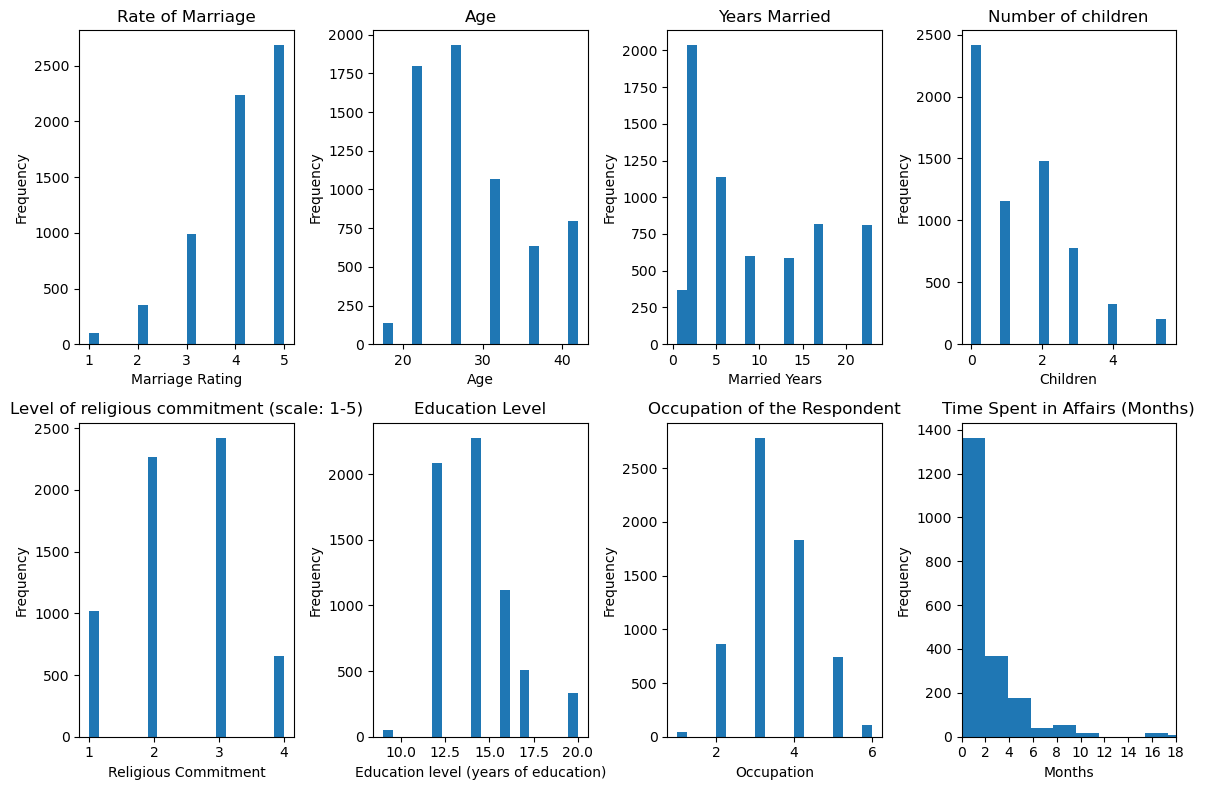
\includegraphics[width=0.85\textwidth]{_assets/eda.png}
\caption{Distribution of key variables in the affairs dataset.}
\label{fig:eda}
\end{figure}

To better understand potential predictors of affairs, we examined the relationships between affair frequency (time spent in extramarital affairs in months) and several demographic and behavioral characteristics.

\subsection{Education and Affairs}

Average affair frequency varied slightly by education level, suggesting that education alone may not be a strong predictor of affair behavior.

\begin{figure}[H]
\centering
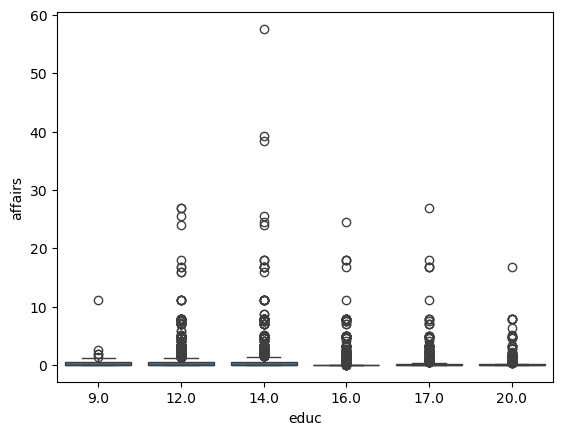
\includegraphics[width=0.48\textwidth]{_assets/affairs_eeducation_boxplot.png}
\hfill
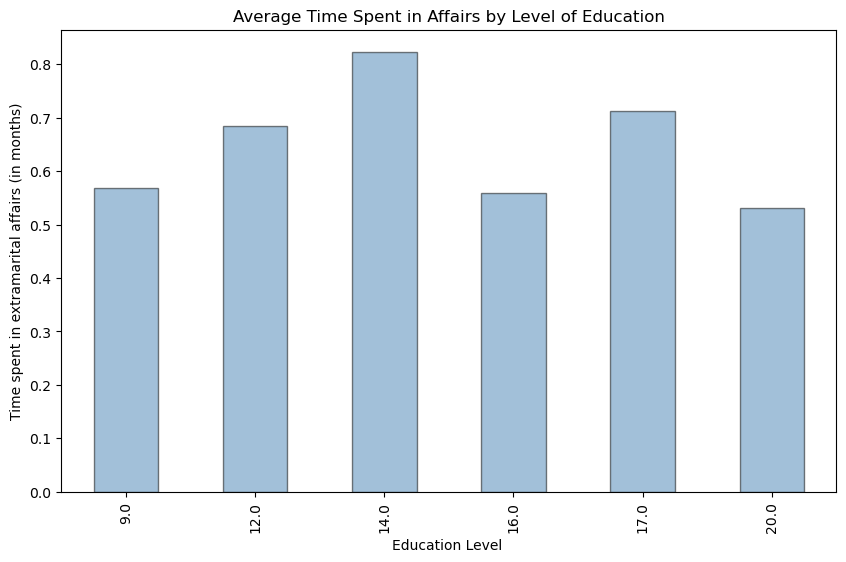
\includegraphics[width=0.48\textwidth]{_assets/avg_affairs_education_plot.png}
\caption{Affair frequency across education levels.}
\label{fig:education}
\end{figure}

\subsection{Religiosity and Affairs}

Respondents with higher levels of religious commitment generally reported fewer affairs. Figure~\ref{fig:religious} shows both the distribution of affair frequency by religious commitment and the corresponding average number of affairs.

\begin{figure}[H]
\centering
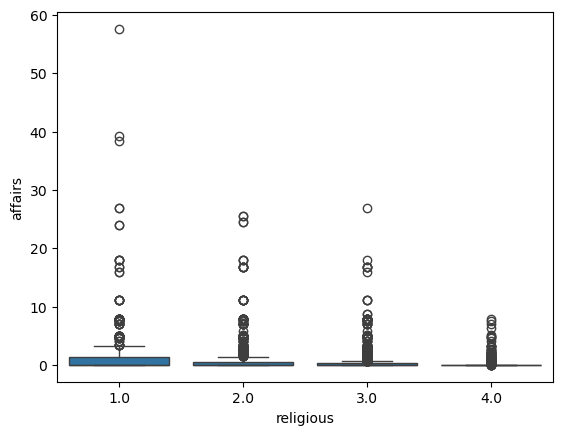
\includegraphics[width=0.48\textwidth]{_assets/affairs_religious_boxplot.png}
\hfill
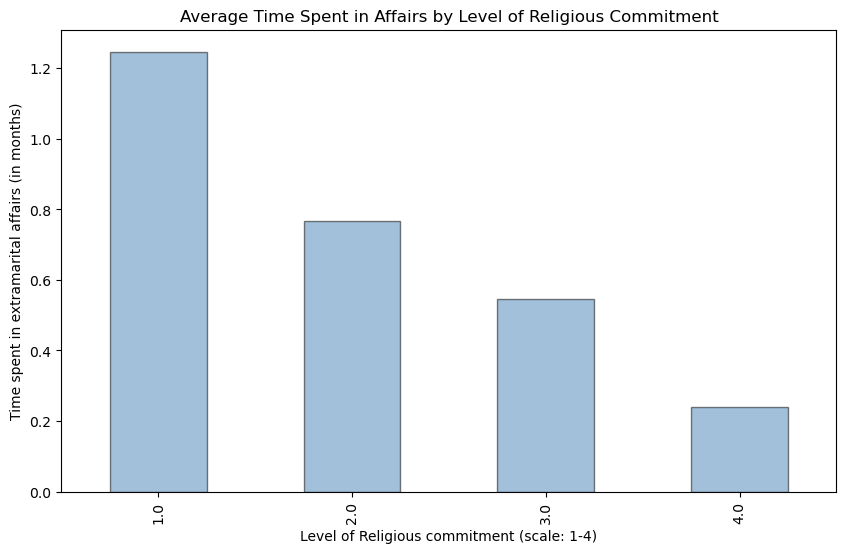
\includegraphics[width=0.48\textwidth]{_assets/affairs_religious_plot.png}
\caption{Relationship between religiosity and affair frequency.}
\label{fig:religious}
\end{figure}

\subsection{Marital Satisfaction and Affairs}

Marital satisfaction exhibited the strongest relationship with affair frequency. Individuals reporting lower levels of marital satisfaction were substantially more likely to report affairs. This relationship suggests that marital satisfaction may be an important predictor in classification models.

\begin{figure}[H]
\centering
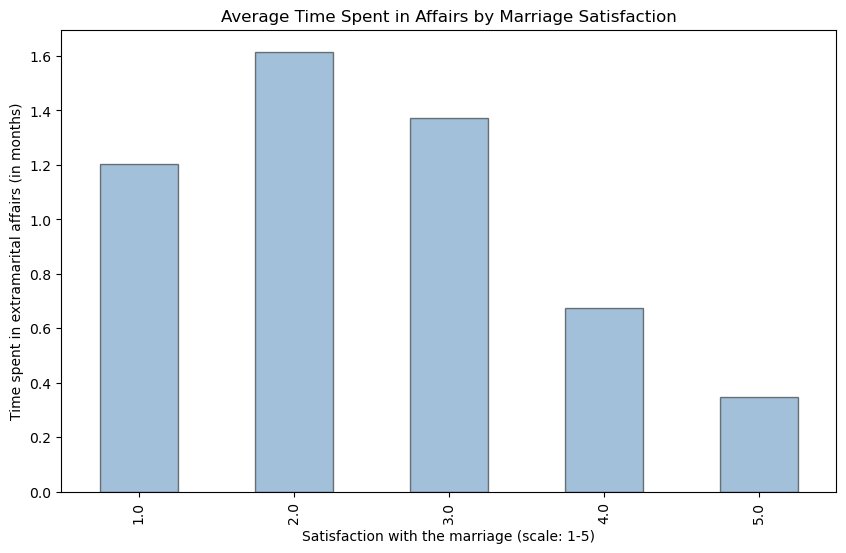
\includegraphics[width=0.7\textwidth]{_assets/affairs_satisfaction.png}
\caption{Relationship between marital satisfaction and affair frequency.}
\label{fig:satisfaction}
\end{figure}

\section{Data Processing/Cleaning}

\subsection{Feature Engineering}

For visualization and exploratory data analysis purposes, the categorical variables \texttt{occupation} and \texttt{occupation\_husb} were recoded from their original numeric encodings into descriptive occupation categories. These descriptions were obtained from the \href{https://www.statsmodels.org/dev/datasets/generated/fair.html}
{Affairs Dataset}. Specifically, the values were mapped as follows: 1 = Student, 2 = Agriculture, 3 = White Collar, 4 = Teacher/Nurse, 5 = Managerial, and 6 = Professional. The same mapping was applied to both the respondent's occupation and the husband's occupation. The recoded occupation variables were not included in the final predictive models.

\subsection{Target Variable}
The \texttt{affairs} variable is continuous and represents the amount of time spent in extramarital affairs. For classification modeling, a binary target variable was created:

\[
\mathrm{had\_affair} =
\begin{cases}
0, & \text{if affairs} = 0 \\
1, & \text{if affairs} > 0
\end{cases}
\]

where 0 indicates that no affair was reported and 1 indicates that the respondent reported at least one affair.



\section{Modeling}

The objective of this analysis was to predict whether an individual reported an extramarital affair. Using the engineered binary response variable \verb|had_affair|, two classification models were developed and evaluated: Logistic Regression and Decision Tree Classification.

\subsection{Logistic Regression}

As we learned in this course, Logistic Regression is a Generalized Linear Model that models the probability that one of 2 outcomes occurs. The independent variables for the input can be categorical or continuous. In our case of categorical inputs, we used one hot encoding to expand the set of features and estimated the probability that an individual reported an affair. 
Because the response variable was binary, we used logistic regression for modeling the relationship between the predictor variables and the likelihood of affair occurrence.

\[
\log\left(\frac{p}{1-p}\right)
=
\beta_0
+
\beta_1(\text{rate\_marriage})
+
\beta_2(\text{age})
+
\beta_3(\text{yrs\_married})
+
\beta_4(\text{children})
+
\beta_5(\text{religious})
+
\beta_6(\text{educ})
\]

Our model used all features, excluding occupation variables. The predictor variables included marital satisfaction (\verb|rate_marriage|), age (\verb|age|), years married (\verb|yrs_married|), number of children (\verb|children|), religious commitment (\verb|religious|), and education level (\verb|educ|). 

We split the data into a training and testing set of 80\% training and 20\% test data. Our model performance was assessed using overall classification accuracy, a confusion matrix, and a classification report containing precision, recall, and F1-score metrics.

\subsection{Decision Tree Classification}

Next, a decision tree classifier was trained to identify the most important predictors of affair occurrence. Rohit explained, "A decision tree classifier iteratively splits the dataset along one of the features and assigns a label to the region according to majority vote. Unless a region is already all of the same output label, the classifier will continue to subdivide along one of the axes."

The same training and testing partitions used for logistic regression were used to train and evaluate the decision tree model. Splits were selected using the Gini impurity criterion, which measures the degree of class mixing within a node. Lower Gini values indicate purer nodes and improved class separation.

\section{Results}

Both models performed similarly. The logistic regression model achieved an accuracy of 70.96\%, while the decision tree classifier achieved an accuracy of 70.17\%. 

\subsection{Decision Tree Classifier}

Figure~\ref{fig:tree} displays the fitted decision tree. The model identified marital satisfaction (\verb|rate_marriage|) as the most important predictor of affair occurrence, followed by years married (\verb|yrs_married|). Individuals reporting lower marital satisfaction were substantially more likely to be classified as having an affair.

\begin{figure}[H]
\centering
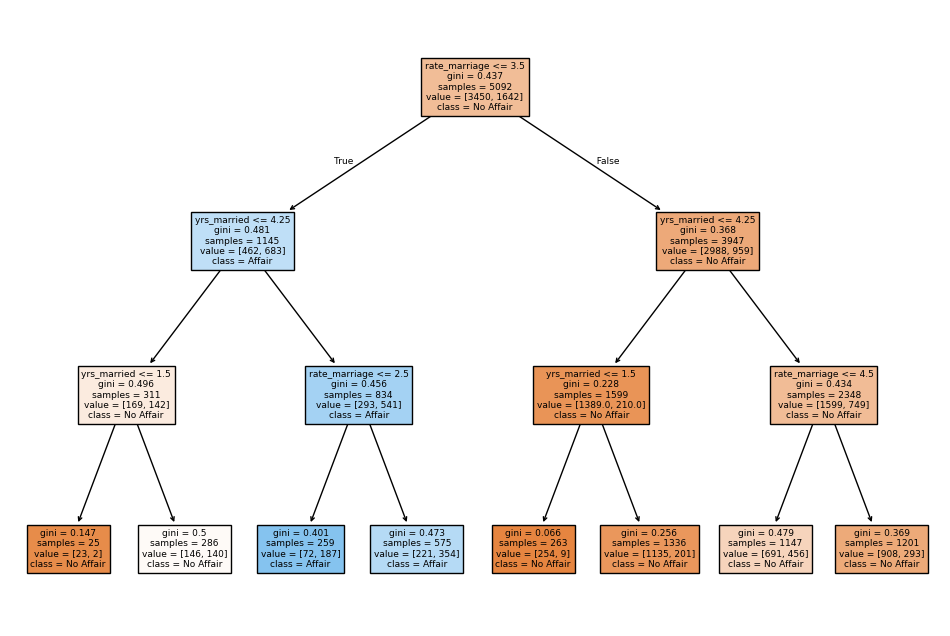
\includegraphics[width=\textwidth]{_assets/Decision_Tree_classifier.png}
\caption{Decision tree classifier predicting affair occurrence.}
\label{fig:tree}
\end{figure}

\subsection{Classification Performance}

Figure~\ref{fig:classification_report} summarizes the classification metrics for the model. The logistic regression model achieved an overall accuracy of 70.96\% on the testing dataset. The "No Affair'' class (precision = 0.742, recall = 0.875, F1-score = 0.803) performed better than the "Affair'' class (precision = 0.588, recall = 0.363, F1-score = 0.446). Of all people who truly had no affair, the model correctly identified 87.5\%. However, the model struggled to detect individuals who reported an affair. The model correctly identified only 36.3\% of the people who actually had an affair. 
\begin{figure}[H]
\centering
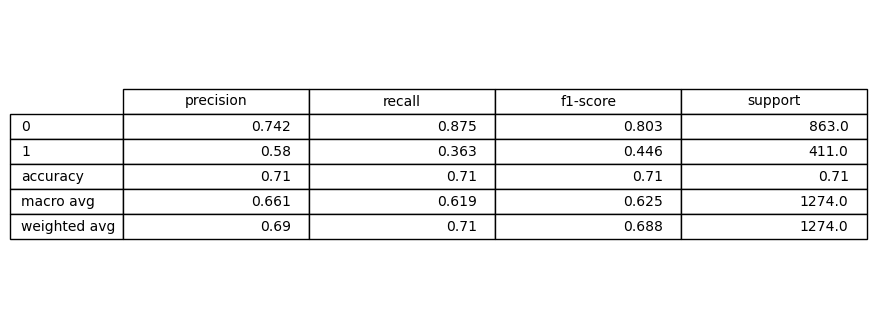
\includegraphics[width=0.8\textwidth]{_assets/classification_report.png}
\caption{Classification report showing precision, recall, F1-score, and support.}
\label{fig:classification_report}
\end{figure}

Overall, both models demonstrated moderate predictive ability. The logistic regression achieved slightly higher predictive accuracy, but the decision tree offered greater interpretability by clearly illustrating how marital satisfaction and years married contributed to affair occurrence.

\section{Challenges}

In retrospect, one of the main challenges was transforming the \verb|affairs| variable into a binary outcome to indicate whether an affair was reported. While this simplification enabled the use of logistic regression and decision tree classification, it resulted in the loss of information regarding the duration of affairs. Alternative modeling approaches, such as multiple linear regression, Poisson regression, or negative binomial regression, could have retained the original continuous \texttt{affairs} variable rather than converting it to a binary outcome.





\end{document}
```
